\documentclass[tikz,border=3mm]{standalone}
\begin{document}
	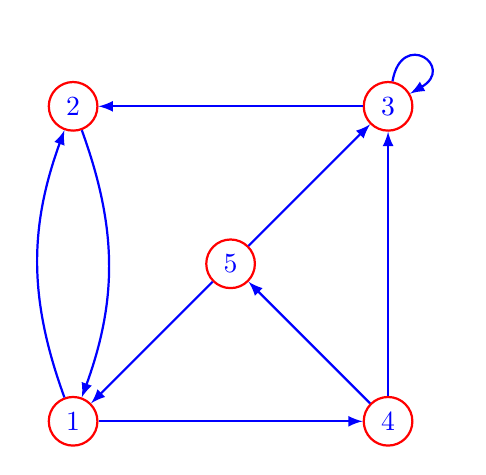
\begin{tikzpicture}
		[every node/.style={circle,draw=red},
		every path/.style={blue,-latex,thick}]
		\def\a{2}
		\node (5) at (0,0) {$5$};
		\node (1) at (-\a,-\a) {$1$};
		\node (2) at (-\a,\a) {$2$};
		\node (3) at (\a,\a) {$3$};
		\node (4) at (\a,-\a) {$4$};
		\draw (1)--(4); \draw (4)--(3);
		\draw (3)--(2); \draw (5)--(3);
		\draw (5)--(1); \draw (4)--(5);
		\draw (2) to[out=-70,in=70] (1);
		\draw (1) to[out=110,in=-110] (2);
		\draw (3) .. controls +(80:1) and +(30:1) .. (3);
	\end{tikzpicture}
\end{document}